\documentclass[aps,twocolumn,secnumarabic,nobalancelastpage,amsmath,amssymb,
nofootinbib,superscriptaddress]{revtex4-1}


\usepackage{graphics}       % standard graphics specifications
\usepackage{graphicx}       % alternative graphics specifications
\usepackage{longtable}      % helps with long table options
\usepackage{url}            % for on-line citations
\usepackage{bm}             % special 'bold-math' package
\usepackage[ngerman]{babel} % deutsche Siblentrennung
\usepackage[utf8]{inputenc} % Umlaute

\def\andname{\hspace*{-0.5em},} % definiert die Trennung zwischen 2 Autoren neu

% Titelseite
\begin{document}
\title{F-Praktikum: Elektrolumineszenz-Spektroskopie}
\author         {Ch. Egerland}
\email[Email: ]{egerlanc@physik.hu-berlin.de}
\author         {M. Pfeifer}
\email[Email: ]{mpfeifer@physik.hu-berlin.de}
\affiliation    {Humboldt-Universität zu Berlin, Institut für Physik}
\date[Versuchsdatum: ]{06.07.2017}

%%%%%%%%%%%%%%%%%%%%%%%%%%%%%%%%%%%%%%%%%%%%%%%%%%%%%%%%%%%%%%%%%%%%%%%%%%%%%%%%
\begin{abstract}
Untersucht wird das Lumineszenzspektrum einer InGaP-Photodiode im Temperaturbereich zwischen
$80\text{ K}$ und $250\text{ K}$. Die Fluoreszenzmessung wird mithilfe eines Czerny-Turner-Spektrometers
und einer Photomultiplier-Tube realisiert. Wir treffen Aussagen über den Verlauf des Spektrums, die
Temperaturabhängigkeit des Lumineszenzpeaks, den thermischen Einluss auf die integrierte Peakintensität und
wir geben eine Abschätzung für die Aktivierungsenergie von InGaP an.
\end{abstract}


\maketitle


%%%%%%%%%%%%%%%%%%%%%%%%%%%%%%%%%%%%%%%%%%%%%%%%%%%%%%%%%%%%%%%%%%%%%%%%%%%%%%%%

\section{Theorie}

\noindent Unter Lumineszenz versteht man Strahlung, die beim Übergang eines Systems von einem angeregten Zustand
in einen niederenergetischen Zustand emittiert wird. Bei Halbleitern lassen sich diese Übergänge mit dem Bändermodell
beschreiben. So finden die elektronischen Übergänge vor allem aus dem Leitungsband ins Valenzband statt, so dass bei
Anregung des Materials mit ausreichend Energie ($E>E_g$) Lumineszenzphotonen mit einer der Bandlücke entsprechenden
Frequenz erzeugt werden (direkter Übergang).\newline

\noindent Es gibt verschiedene Rekombinationswege für ein sich im angeregten Zustand befindlichendes System (s. \ref{fig:rekomb} ) \cite{saarland}.
Liegt ein dotierter Halbleiter vor, speziell z.B. eine Heterostruktur mit pn-Übergang, gibt es im Bereich zwischen Leitungs-
und Valenzband Donator- (knapp unter Leitungsbandkante) und Akzeptorzustände (knapp über der Valenzbandkante). Ebenfalls für die
Lumineszenz relevant sind sog. Exzitonen-Zustände (gebundene Elektron-Loch-Paare). Bei guter Kühlung (wenig thermischer
Anregung) sind neben dem direkten Übergang (LB$\rightarrow$VB) daher auch andere Übergänge, z.B. Exzitonen-Rekombination,
Übergänge vom Donator- zum Akzeptorniveau (D,A) oder ins Valenzband (D,h) sichtbar.

\begin{figure}[h!]
  \centering
  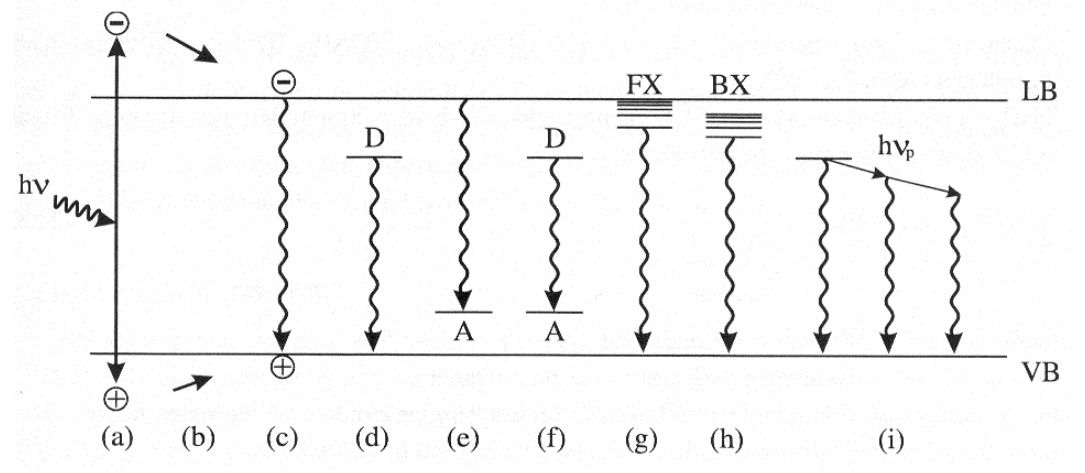
\includegraphics[width=0.47\textwidth]{img/rekombinationswege.jpg}
  \caption{ Lumineszenz-relevante elektronische Übergänge: a) Anregung, b) Relaxation im Band,
  c) (e,h)-Übergang, d) (D,h)-Übergang, e) (e,A)-Übergang, f) (D,A)-Übergang, g) Rekombination freier Exzitonen; aus: \cite{saarland}}
  \label{fig:rekomb}
\end{figure}


%%%%%%%%%%%%%%%%%%%%%%%%%%%%%%%%%%%%%%%%%%%%%%%%%%%%%%%%%%%%%%%%%%%%%%%%%%%%%%%%

\section{Experiment}

\noindent Der Versuchsaufbau ist schematisch in \ref{fig:versuch} dargestellt. Die Anregung der InGaP-Diode erfolgt durch Anlegen einer
Spannung mittels einer externen Konstantstromversorgung. Dazu sind die elektrischen Verbindungen bereits an der Probe angebracht.
Diese befindet sich in einem evakuierten ($p\sim 2\text{ Pa}$) und auf $80\text{ K}$ Stickstoff-temperierten Kryostaten. Die Temperaturmessung
erfolgt durch einen Sensor, der möglichst nahe an der Probe platziert wurde.

\begin{figure}[h]
  \centering
  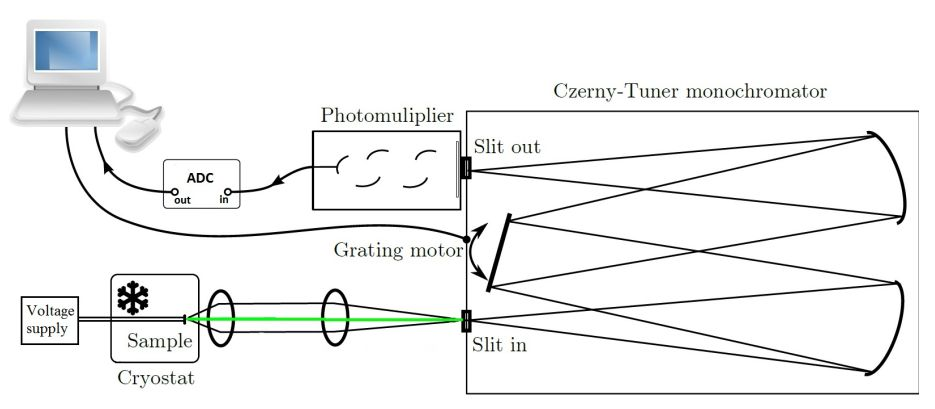
\includegraphics[width=0.48\textwidth]{img/versuchsanleitung.jpg}
  \caption{Versuchsaufbau, aus: \cite{anleitung}}
  \label{fig:versuch}
\end{figure}

\noindent Die durch Rekombination entstandenen Photonen gelangen zunächst durch eine Kollimatorlinse, gefolgt von einer Linse zur
Strahlfokussierung und treffen dann auf ein Czerny-Turner-Monochromator. Durch die Beweglichkeit des Gitters im
Monochromator (Schrittmotorsteuerung) können verschiedene Spektralbereiche selektiert werden, deren Intensität anschließend in einem Photomultiplier (PMT)
gemessen wird. Dieser arbeitet mit einer Beschleunigungsspannung von $U_\text{PMT}=2,2\text{ kV}$. Zwecks Maximierung des
Signal-Rausch-Verhältnisses wurde die PMT ebenfalls gekühlt (Peltierelement mit Wasserkühlung). Das Signal der Photonenvervielfachers
gelangt dann über einen Analog-Digital-Wandler zum Computer, der die Messsignale zusammen mit der Schrittmotorposition des Monochromators
abspeichert und zu einem Energiespektrum verarbeitet.

Hier mal noch Beispiele wie man Gleichungen richtig referenziert, siehe
Gleichung.~\ref{eq:first-equation} :
\begin{equation}
   \chi_+(p)\alt{\bf [}2|{\bf p}|(|{\bf p}|+p_z){\bf ]}^{-1/2}
   \left(
   \begin{array}{c}
      |{\bf p}|+p_z\\
      px+ip_y
   \end{array}\right)
   \label{eq:first-equation}
\end{equation}


Oder auch in der Zeile: $\vec{\psi_1} = |\psi_1\rangle \equiv c_0|0\rangle +
c_1|1\rangle \chi^2 \approx
\prod\sum\left[\frac{y_i-f(x_i)}{\sigma_i}\right]^2 |\psi_1\rangle
\sim \lim_{\mu \rightarrow \infty}p(x;\mu) \geq \frac{1}{\sqrt{2 \pi
\mu}} e^{-(x-\mu)^2 / 2\mu}P(x) \ll \int_{-\infty}^x p(x')dx'a
\times b \pm c \Rightarrow \nabla \hbar$.

Manchmal auch über mehr als eine Zeile, siehe Equation~\ref{eq:multilineeq}:
\begin{eqnarray}
  \sum \vert M^{\text{viol}}_g \vert ^2
   &=&  g^{2n-4}_S(Q^2)~N^{n-2} (N^2-1)
\nonumber
\\
   &&   \times \left( \sum_{i<j}\right) \sum_{\text{perm}}
            \frac{1}{S_{12}}  \frac{1}{S_{12}} \sum_\tau c^f_\tau
\,.
\label{eq:multilineeq}
\end{eqnarray}

Natürlich gibts auch die guten alten subequations wie (\ref{subeq:1}) und
(\ref{subeq:2}):
\begin{subequations}
\label{eq:whole}
\begin{equation}
  \left\{
      abc123456abcdef\alpha\beta\gamma\delta1234556\alpha\beta
       \frac{1\sum^{a}_{b}}{A^2}
  \right\}
%
\,\label{subeq:1}
\end{equation}
\begin{eqnarray}
  {\cal M} &=& ig_Z^2(4E_1E_2)^{1/2}(l_i^2)^{-1}
                (g_{\sigma_2}^e)^2\chi_{-\sigma_2}(p_2)
\nonumber\\
  &&\times [\epsilon_i]_{\sigma_1}\chi_{\sigma_1}(p_1).\label{subeq:2}
\end{eqnarray}
\end{subequations}




%%%%%%%%%%%%%%%%%%%%%%%%%%%%%%%%%%%%%%%%%%%%%%%%%%%%%%%%%%%%%%%%%%%%%%%%%%%%%%%%
\section{Daten und Analyse}

Lorem ipsum dolor sit amet, consectetur adipiscing elit. Nam id facilisis ligula,
a ultrices nibh. Nullam suscipit tellus nec mauris fermentum, ornare luctus neque
tincidunt. Aenean commodo tincidunt varius. Phasellus faucibus metus non erat
consectetur bibendum. Duis et luctus risus, at egestas justo. Nunc eleifend lacus
ac laoreet scelerisque. Aenean cursus dignissim magna in ultrices. In eget nisl
quis nisi. Tabelle \ref{tab:table1}:


\begin{table}[h]
\caption{\label{tab:table1}Eine Tabelle mit Fußnoten}
\begin{ruledtabular}
\begin{tabular}{cccccccc}
 &$r_c$ (\AA)&$r_0$ (\AA)&$\kappa r_0$&
 &$r_c$ (\AA) &$r_0$ (\AA)&$\kappa r_0$\\
\hline
Cu& 0.800 & 14.10 & 2.550 &Sn\footnotemark[1] & 0.680 & 1.870 & 3.700 \\
Ag& 0.990 & 15.90 & 2.710 &Pb\footnotemark[1] & 0.450 & 1.930 & 3.760 \\
Tl& 0.480 & 18.90 & 3.550 & & & & \\
\end{tabular}
\end{ruledtabular}
\footnotetext[1]{Entnommen aus Ref.~\cite{bevington2003}.}
\end{table}




%%%%%%%%%%%%%%%%%%%%%%%%%%%%%%%%%%%%%%%%%%%%%%%%%%%%%%%%%%%%%%%%%%%%%%%%%%%%%%%%
\section{Schlussfolgerung}

Schlussoflgerung, sollten wir mal was von nem Buch oder so entnehmen nutzen wir:


\begin{quote}
  Ein Zitat mit Referenz auf das Buch\cite{melissinos1966}
\end{quote}

Lorem ipsum dolor sit amet, consectetur adipiscing elit. Nam id facilisis ligula,
a ultrices nibh. Nullam suscipit tellus nec mauris fermentum, ornare luctus neque
tincidunt. Aenean commodo tincidunt varius. Phasellus faucibus metus non erat
consectetur bibendum. Duis et luctus risus, at egestas justo. Nunc eleifend lacus
ac laoreet scelerisque. Aenean cursus dignissim magna in ultrices. In eget nisl
quis nisi.


%%%%%%%%%%%%%%%%%%%%%%%%%%%%%%%%%%%%%%%%%%%%%%%%%%%%%%%%%%%%%%%%%%%%%%%%%%%%%%%%
\bibliography{sample-paper}
\bibliographystyle{prsty}
\begin{thebibliography}{99}
\bibitem{saarland}Prof. Dr. Thomas Wichert, Photolumineszenz-Spektroskopie an Halbleitern, Universität des Saarlandes [2006]
\bibitem{anleitung}FET Group, Benutzerhandbuch Elektrolumineszenz-Spektroskopie, Humboldt-Universität zu Berlin
\bibitem{abkuerzung3}Autor, Titel, Verlag,  [1945]
\bibitem{abkuerzung4}Autor, Titel, Verlag,  [1945]
\end{thebibliography}


%%%%%%%%%%%%%%%%%%%%%%%%%%%%%%%%%%%%%%%%%%%%%%%%%%%%%%%%%%%%%%%%%%%%%%%%%%%%%%%%
\clearpage
\appendix

\section{Sonstiges}
Hier sehen wir einen Beispiel Anhang und so könnte man Code in Latex einbinden:
\begin{verbatim}
> mkdir ~/8.13
> mkdir ~/8.13/papers
> mkdir ~/8.13/papers/template
> cd ~/8.13/papers/template
\end{verbatim}


%%%%%%%%%%%%%%%%%%%%%%%%%%%%%%%%%%%%%%%%%%%%%%%%%%%%%%%%%%%%%%%%%%%%%%%%%%%%%%%%


\end{document}
